% !TeX program = xelatex

% 页面设置
\documentclass[12pt]{article}
\usepackage[a4paper, margin=2cm]{geometry}

% 中文排版
\usepackage[fontset=none]{ctex}

% 字体
\setmainfont{LinLibertineO}[BoldFont=LinLibertineOB]
\setCJKmainfont{FZNewShuSong-Z10}[BoldFont=FZXiaoBiaoSong-B05]

% 标题样式
\usepackage{titlesec}
\titleformat{\section}{\Large\bfseries}{\chinese{section}、}{0em}{}

% 图表
\usepackage{graphicx}
\usepackage{xcolor}
\usepackage{tikz}
\usetikzlibrary{calc, fit, positioning, shapes.geometric}

% 链接样式
\usepackage{hyperref}
\hypersetup{colorlinks, linkcolor=[cmyk]{0.55,1,0,0.15}, urlcolor=[cmyk]{1,0.58,0,0.21}}
\urlstyle{same}
\def\UrlBreaks{\do\/\do-}

\newcommand{\footnotep}[1]{\hskip -0.5em\footnote{#1}\hskip 0.5em}

\begin{document}

% 标题
\null
\begin{center}
  \Large 程序设计实习\quad Qt 大作业 \vskip 0.5em
  \LARGE \textbf{作业报告} \vskip 1em
  \large 王韦煊\quad 侯旭森\quad 郑世淇 \vskip 0.5em
  第 31 组 \vskip 0.5em
  2023 年 7 月 8 日 \vskip 1.5em
\end{center}

% 正文
\section{程序功能介绍}

\begin{figure}[p]
  \centering
  \vskip -2em
  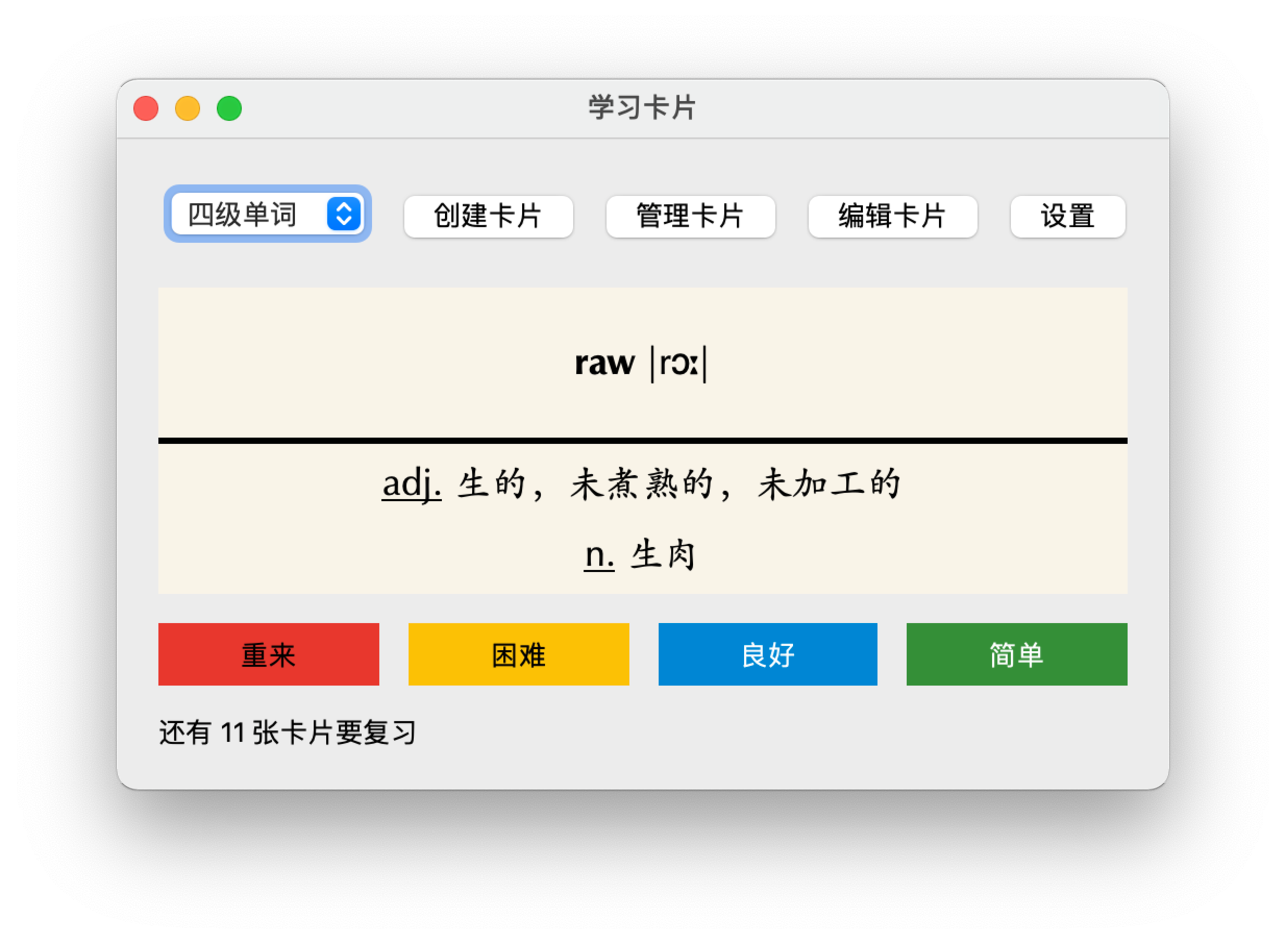
\includegraphics[scale=0.44]{fig/screenshot-study.pdf}
  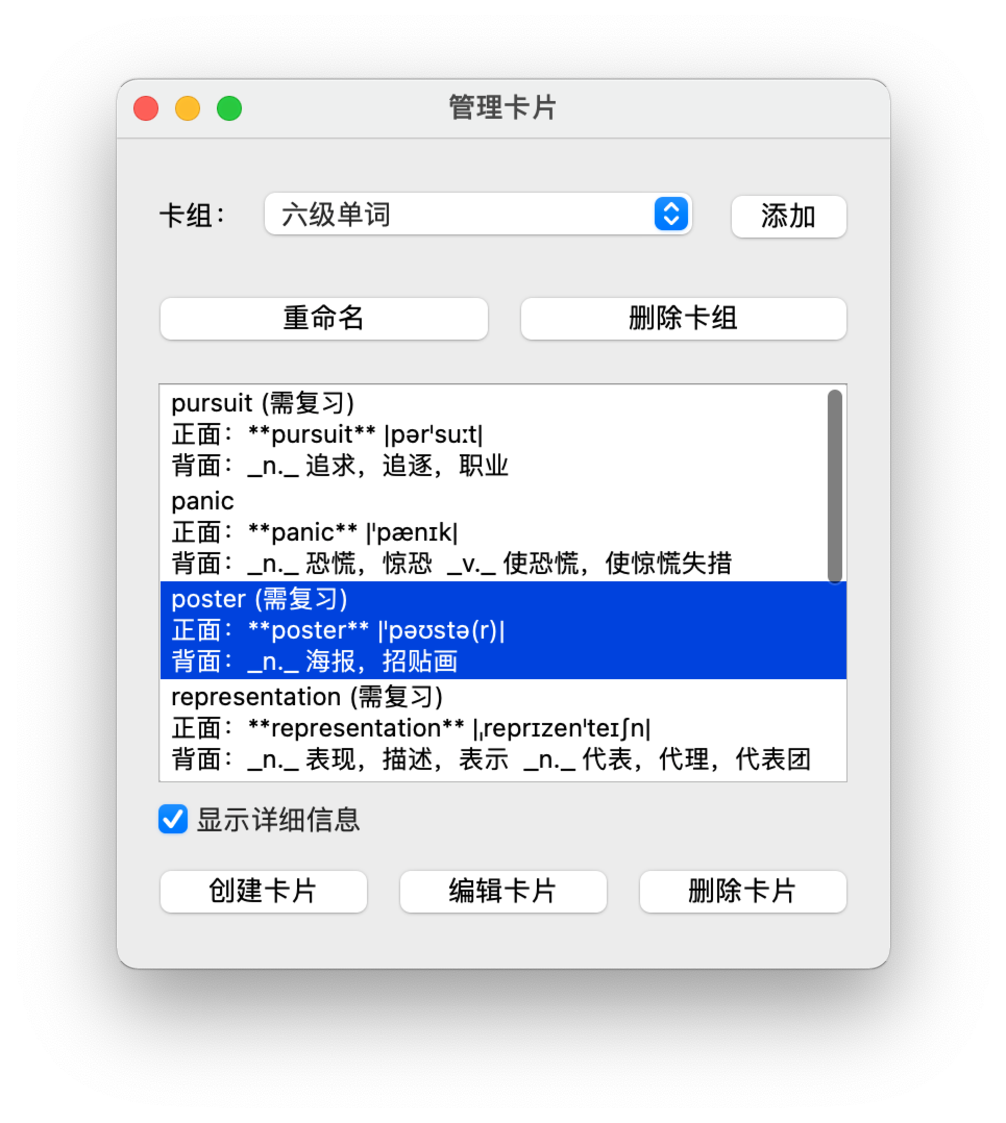
\includegraphics[scale=0.44]{fig/screenshot-manager.pdf}
  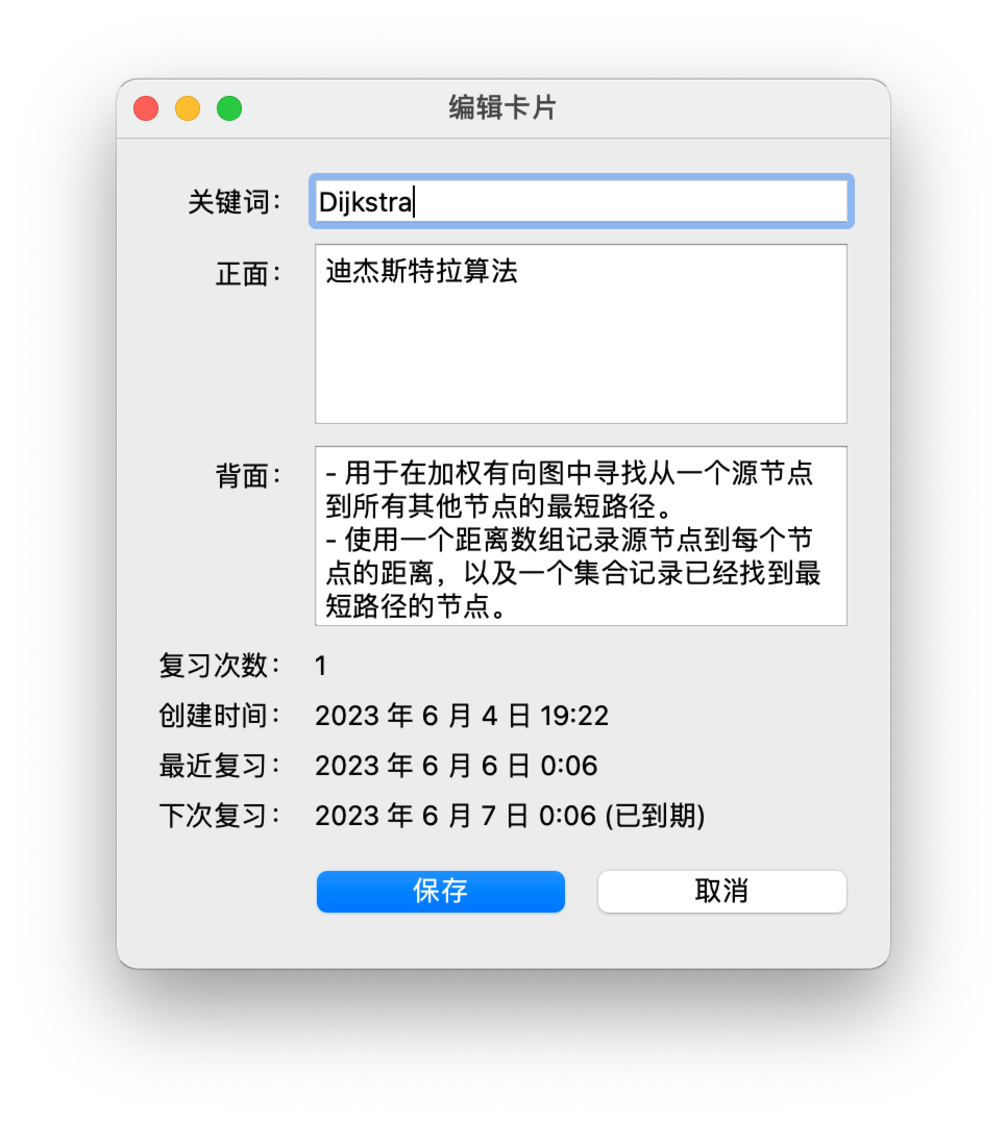
\includegraphics[scale=0.44]{fig/screenshot-editor.pdf}
  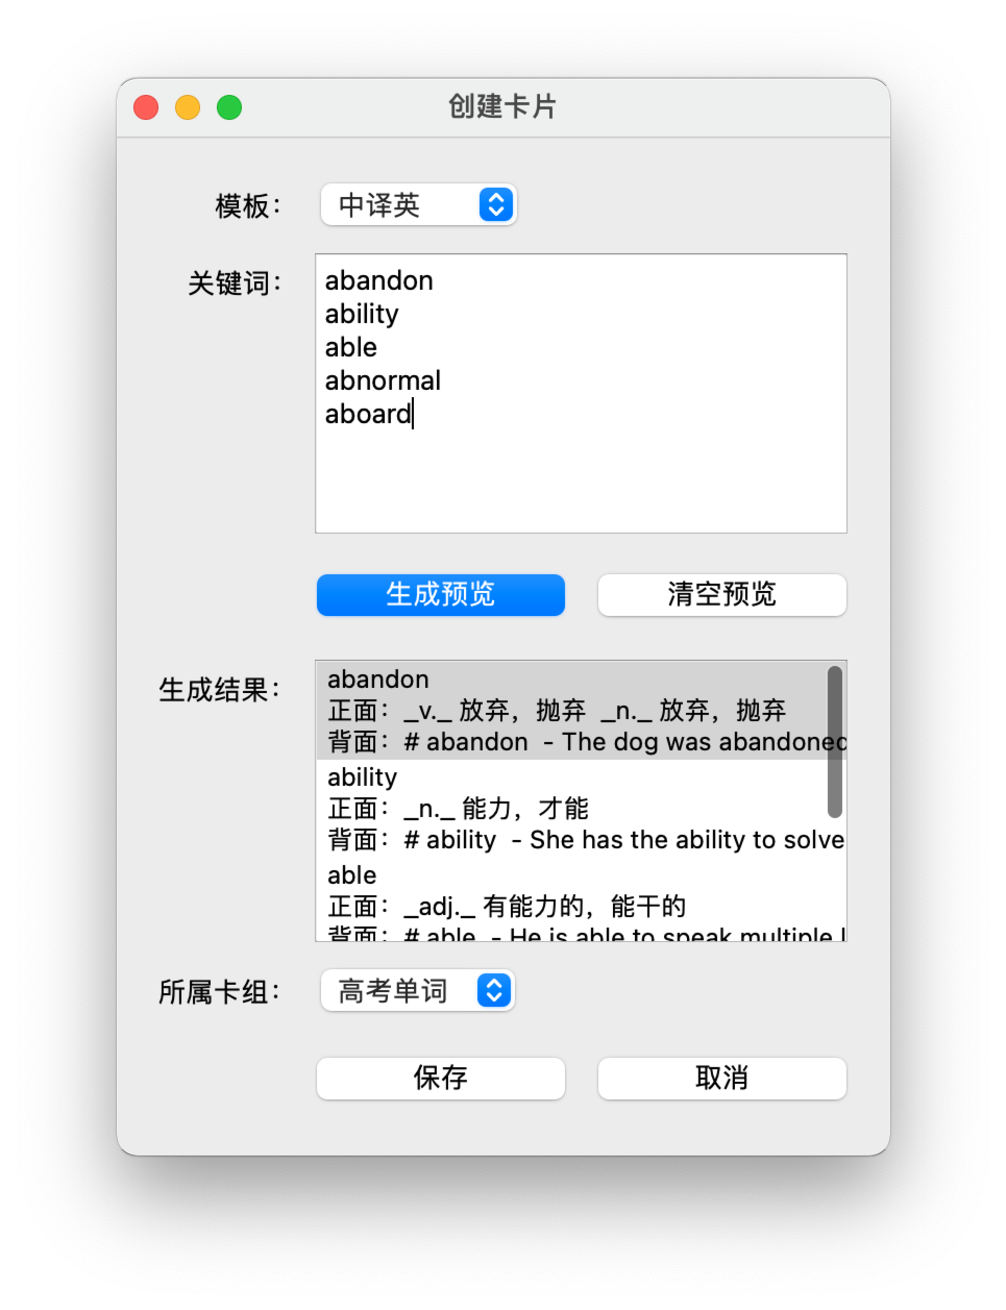
\includegraphics[scale=0.44]{fig/screenshot-composer.pdf}
  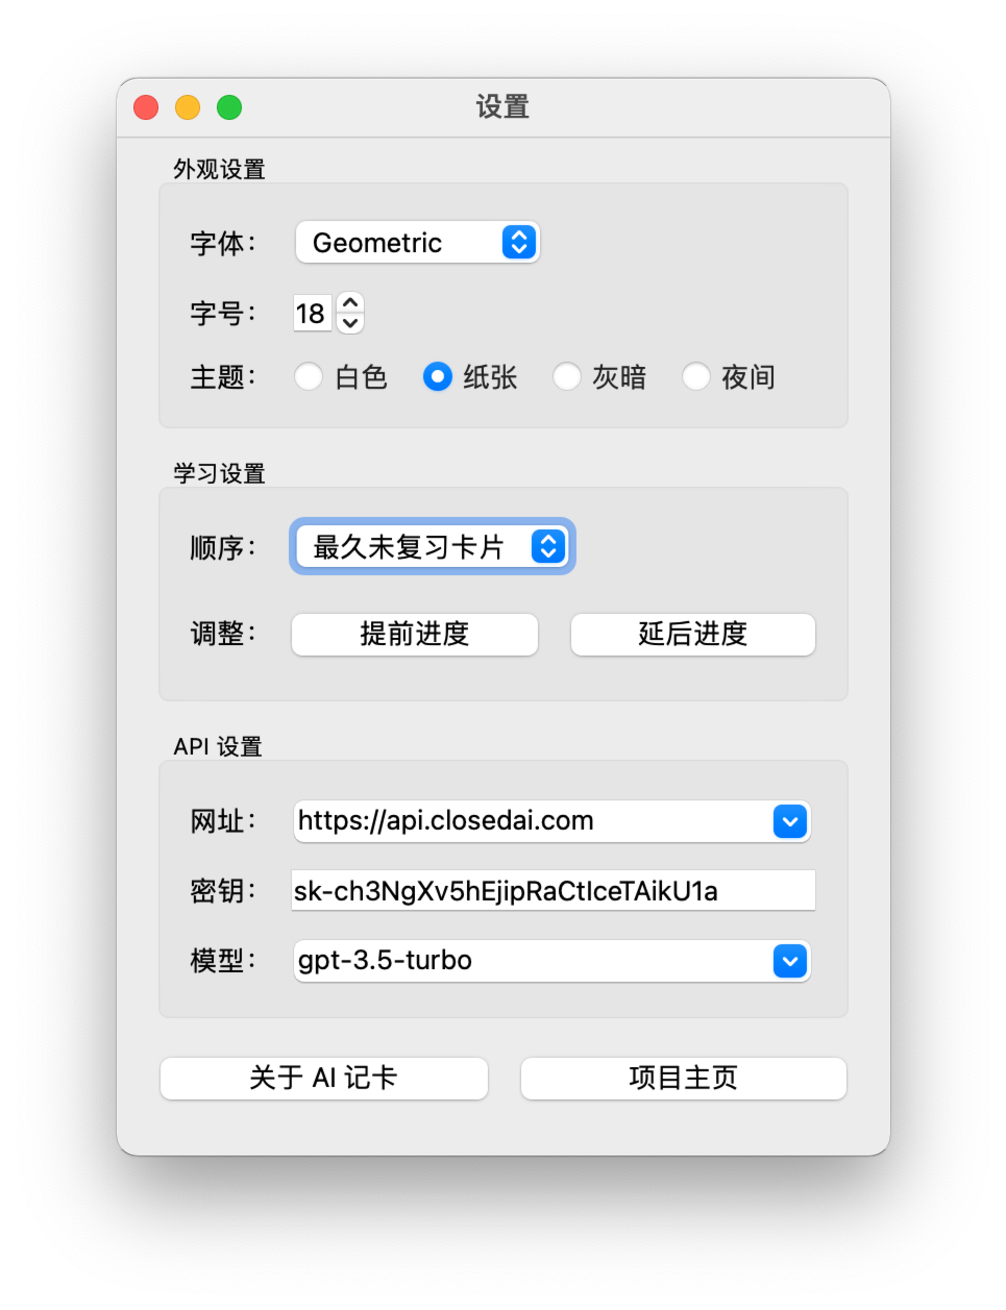
\includegraphics[scale=0.44]{fig/screenshot-settings.pdf}
  \vskip -1em
  \caption{程序界面}\label{fig:screenshots}
\end{figure}

本组的 Qt 大作业为一款紧随时代的记忆卡片软件,\footnotep{\url{https://github.com/wangweixuan/pkupop-term-project}} 名为《AI 记卡》,界面简洁,功能强大。程序基于间隔重复算法,可以自动安排卡片的复习计划,帮助用户记忆。此外,软件可根据用户提供的关键词,利用生成式语言模型,批量生成记忆卡片。

如图 \ref{fig:screenshots} 所示,本软件有五个窗口。“学习卡片”为主窗口,其设计借鉴了 Anki 应用。\footnotep{\url{https://apps.ankiweb.net/}} 单词以“卡片”的形式呈现,正面为“问题”,背面为“答案”,均支持 Markdown 富文本内容。用户可自主选择是否查看答案,并根据自己对卡片的熟悉程度提供反馈。软件还支持自定义卡片的字体字号、颜色主题。若干张卡片组成“卡组”,复习卡片时将轮流展示选定卡组中的卡片。软件的其他窗口提供了管理卡片与卡组、创建卡片、编辑卡片等功能。

程序跟踪卡片的学习历史、难易程度等属性,内置了基于 SuperMemo 间隔重复算法\footnote{\url{https://super-memory.com/english/ol/sm2.htm}} 的三种复习模式,自动筛选和排序需要复习的卡片,并提供了提前进度和延后进度的选项,保证了背诵的科学和效率。所有卡片数据自动保存和恢复,适合长期使用。

软件可以按指定的关键词自动生成记忆卡片。它以 ChatGPT 所用的大语言模型为内容生成的基础,轻松适应不同领域、不同用途、不同语言的单词生成,打破了单词软件对传统字典的依赖,空前提高了单词软件的灵活性。无论是对于传统的两种语言之间的单词背诵,如“英译中”“中译英”,还是基于大模型开发的新场景,如“C++ 概念”“算法概念”“智慧问答”,这款软件都可以轻松实现对给定关键词的卡片生成,从而组建相应的卡组。

\section{项目各模块与类设计细节}

\subsection{程序架构}

程序架构如图 \ref{fig:structure-chart} 所示,包含用户界面模块、公共模块、数据模型模块、卡片生成器模块。

main 函数创建全局状态并启动“学习卡片”窗口。在首次使用程序(数据库为空)时,还会显示欢迎界面。全局状态通过构造函数注入到用户界面各个组件。

\begin{figure}[t]
  \centering
  \tikzset{
  label/.style = {
      align = center,
      node distance = 2mm,
    },
  class/.style = {
      rectangle,
      align = center,
      ultra thick,
      minimum width = 30mm,
      node distance = 5mm,
    },
  resource/.style = {
      trapezium,
      trapezium left angle = 60,
      trapezium right angle = 120,
      trapezium stretches = true,
      align = center,
      ultra thick,
      minimum width = 30mm,
      node distance = 5mm,
    },
  frame/.style = {
      rounded corners = 5mm,
      inner sep = 4mm,
      ultra thick,
      dashed,
    },
  service/.style = {
      ellipse,
      align = center,
      ultra thick,
      node distance = 5mm,
    },
  relation/.style = {
      ->,
      ultra thick,
    },
  ui/.style = {
      draw = magenta,
    },
  common/.style = {
      draw = blue!80!white,
    },
  common text/.style = {
      text = blue!80!white,
    },
  model/.style = {
      draw = orange!80!black,
    },
  model text/.style = {
      text = orange!80!black,
    },
  gen/.style = {
      draw = green!50!black,
    },
  gen text/.style = {
      text = green!50!black,
    },
}
\begin{tikzpicture}
  \node (main) {
    main
  };
  \node[ui,class,right=of {[yshift=-0.8em]$(main.east)$},minimum width=35mm] (windows) {
      窗口\\
      StudyWindow\\
      ManagerWindow\\
      SettingsWindow
    };
  \node[ui,class,below=3mm of windows,minimum width=35mm] (dialogs) {
    对话框\\
    ComposerDialog\\
    EditorDialog
  };
  \node[label,above=of windows] (ui label) {
    用户界面\\
    ui
  };
  \node[ui,frame,fit=(ui label)(dialogs)] (ui frame) {};
  %
  \node[common,common text,class,below right=12mm and -10mm of dialogs.south west] (globals) {
    全局状态\\
    AppGlobals
  };
  \node[common,common text,class,right=of globals] (settings) {
    设置\\
    AppSettings
  };
  \node[common,resource,below=of globals] (db file) {
    数据库文件
  };
  \node[common,resource,below=of settings] (settings file) {
    设置文件
  };
  \node[common,frame,fit=(globals)(settings)(settings file)] (common frame) {};
  %
  \node[model,model text,class,left=12mm of globals] (card db) {
    卡片数据库\\
    CardDatabase
  };
  \node[model,class,above=8mm of card db] (card pack) {
    卡组\\
    CardPack
  };
  \node[model,class,above=8mm of card pack] (card) {
    卡片\\
    Card
  };
  \node[label,above=of card] (card label) {
    数据模型\\
    model
  };
  \node[model text,right=0mm of {$(card db.north)!0.5!(card pack.south)$}] (db vector) {
    vector
  };
  \node[model text,right=0mm of {$(card pack.north)!0.5!(card.south)$}] (pack vector) {
    vector
  };
  \node[model,frame,fit=(card label)(card db)] (card frame) {};
  %
  \coordinate (prompts blc) at ([xshift=12mm]$(dialogs.south east)$);
  \node[gen,resource,anchor=bottom left corner,at=(prompts blc)] (prompts) {
    预设模板
  };
  \coordinate (prompt sw) at ($(prompts blc)+(prompts.north)-(prompts.south)$);
  \node[gen,class,above right=5mm and 0mm of prompt sw,minimum width=20mm] (prompt) {
    模板\\
    Prompt
  };
  \node[gen,class,right=of prompt] (api) {
    API 客户端\\
    ApiManager
  };
  \node[gen,gen text,class,above=of {$(prompt.north)!0.5!(api.north)$}] (generator) {
      卡片生成器\\
      CardGenerator
    };
  \node[gen,frame,fit=(generator)(prompts blc)(api)] (gen frame) {};
  \node[below=20mm of api] (network library) {
    Qt::Network 库
  };
  \node[gen,service,below=of network library] (ai) {
    OpenAI
  };
  %
  \draw[relation] (main) -- ([xshift=10mm]$(main.east)$);
  \draw[relation] (main) to [bend right=20] (globals);
  \draw[ui,relation] ([yshift=-2mm]$(dialogs.south)$) to [bend right=20] (globals);
  \draw[ui,relation] ([xshift=-3mm]$(dialogs.east)$) to [bend left=20] (generator);
  \draw[common,relation] (globals) -- (settings);
  \draw[common,relation] (globals) -- (db file);
  \draw[common,relation] (globals.south east) -- (settings file.west);
  \draw[common,relation] (globals) -- (card db);
  \draw[model,relation] (card db) -- (card pack);
  \draw[model,relation] (card pack) -- (card);
  \draw[gen,relation] (generator) -- (prompt);
  \draw[gen,relation] (generator) -- (api);
  \draw[gen,relation] (prompt) -- (prompts);
  \draw[gen,relation] (api) -- (network library);
  \draw[gen,relation] (network library) -- (ai);
\end{tikzpicture}

  \caption{程序架构。主要的类由方框标出}\label{fig:structure-chart}
\end{figure}

\subsection{用户界面模块}

用户界面包括五个窗口,继承自 QWidget 或 QDialog,具体功能如下:

\begin{itemize}
  \item “学习卡片”窗口 StudyWindow 是主界面,通过按钮与其他窗口和对话框连接。该界面的功能是显示卡片、切换卡片答案、收集用户对卡片记忆程度的反馈、显示复习进度;
  \item “管理卡片”窗口 ManagerWindow 允许用户操作卡组列表以及卡组中的卡片;
  \item “设置”窗口 SettingsWindow 包含设置以及项目主页链接;
  \item “创建卡片”对话框 ComposerDialog 将输入的卡片模板和卡片关键词传递给卡片生成器模块(见 \ref{sec:generator} 节),可批量生成并预览卡片,将新卡片添加到数据库;
  \item “编辑卡片”对话框 EditorDialog 允许用户编辑卡片的关键词及内容,查看卡片详细信息,如复习次数、下次复习时间。
\end{itemize}

此外,共享组件 PackCombo 类对 QComboBox 进行了包装,实现了卡组下拉选择列表,减少了不同窗口间的代码重复。

在视图方面,采用了命令式写法(无 QML),运用 Qt 对象树管理组件的生命周期。运用 QBoxLayout 和 QFormLayout 管理布局。“学习卡片”窗口运用了 QSplitter、QScrollArea、QStackedLayout 展示卡片的正面和背面,并用 Qt 样式表动态设置其字体和颜色。“管理卡片”和“创建卡片”窗口运用了 QListWidget 展示列表。\footnotep{区别于 MVC 模式,我们没有将控制器与视图类分离,以简化开发。参考 \url{https://doc.qt.io/qt-6/model-view-programming.html}}

在数据模型方面,用户界面通过 AppGlobals 类(见 \ref{sec:common} 节)访问卡片数据库和程序设置。各个窗口均运用 Qt 信号机制监听数据和设置的修改,在必要时对视图进行更新。

\subsection{公共模块}\label{sec:common}

程序的所有全局状态记录在 AppGlobals 类中,该类的实例持有卡片数据库(见 \ref{sec:model} 节)和程序设置。

程序设置记录在 AppSettings 类,含数值、字符串、枚举等字段类型。一是外观设置,可综合成 Qt 样式表;二是学习设置,即卡片复习的顺序;三是 API 设置,用于卡片生成器。设置值在更新时进行效验,并利用 Qt 信号机制通知相关组件。

AppGlobals 类还负责数据库和设置的持久化。该类的 Restore 方法从文件读取数据库和设置,由 main 函数调用;Save 方法将数据保存到文件,利用信号机制,在数据库和设置更新时自动调用。文件位置通过 QStandardPaths 确定。

\subsection{数据模型模块}\label{sec:model}

卡片数据模型分为 Card、CardPack、CardDatabase 三层。卡片类 Card 记录了卡片关键词、内容、复习记录,可以直接展示在用户界面。卡组类 CardPack 即卡片的列表,卡片数据库类 CardDatabase 又是卡组的列表。每个卡片和卡组实例均通过数据库分配了整数唯一标识符。

本模块实现了 SuperMemo 间隔重复算法与复习算法。其中,Card 类记录了卡片的复习次数、复习时间、复习间隔、难易因数等属性,包含判断卡片状态的方法、根据用户反馈更新状态的方法。CardPack 类包含按多种复习方案筛选卡片、排序卡片的方法,如“选择最久未复习卡片”“选择最早到期卡片”“随机选择卡片”。

用户界面通常通过整数标识符来访问卡片。CardDatabase 类提供了增删改查的接口,并负责在卡片、卡组、卡组列表发生修改时,利用 Qt 信号机制通知其使用者,以保证数据模型与界面的一致性。

数据模型利用 QList 和 STL 来操作列表,基于 QDataStream 实现序列化及反序列化。

\subsection{卡片生成器模块}\label{sec:generator}

卡片生成器负责利用大语言模型,根据用户输入的关键词和模板来生成卡片。主要的类是 CardGenerator,“创建卡片”对话框依赖于这个类。该类的 Generate 方法可将关键词和所选的模板合成为语言模型的输入,并将请求发送给 OpenAI 等服务。语言模型的响应被解析成结构化的卡片,利用 Qt 信号机制异步地返回到用户界面。

卡片模板由 Prompt 类表示,包含对语言模型的指令(system message),以及卡片示例(few-shot prompting),这两者保证了语言模型在输出格式和输出内容上的可靠性。程序预设了若干种模板,以 JSON 形式存储,在运行时加载。

语言模型交互由 ApiManager 类实现。该类包装了 OpenAI 发布的 chat completions API,\footnotep{\url{https://platform.openai.com/docs/guides/gpt/chat-completions-api}} 根据设置中的 API 网址等参数,通过 Qt::Network 库访问相关服务。整个流程涉及两轮 JSON 序列化及反序列化,妥善处理了网络异常、API 异常、JSON 格式错误等情况。

\subsection{支持模块}

除代码外,软件还包含一些支持文件。基于 CMake 配置了软件的构建系统。利用 Qt 部署工具(windeployqt、macdeployqt)进行打包,对于 Windows 平台利用 InnoSetup 制作安装程序。配置了 GitHub Actions 实现持续集成。

在软件质量方面,已将 clang-format 及 clang-tidy 应用于全部代码。配置了 GoogleTest 框架进行单元测试,覆盖了公共模块、数据模型模块和卡片生成器模块。

此外,还为软件设计了一个图标。\footnotep{图标在 Windows 平台上似乎未生效,原因不明。}

\section{小组成员分工情况}

我们三人共同参与了项目创意讨论、功能设计、路演的准备,以及本报告的编写。组长王韦煊统筹项目开发。在代码方面,郑世淇完成了用户界面模块中较复杂的三个窗口;侯旭森完成了数据模型模块,以及用户界面中的“学习卡片”窗口和共享组件;王韦煊完成了卡片生成器模块和程序设置相关部分。

\begin{figure}[ht]
  \centering
  \NewDocumentCommand { \nodelabel } { m m m m } {
  \node[label={[text=black!60]#4:#1}] at (#2:#3) {};
}
\NewDocumentCommand { \nodetext } { m m m } {
  \node[align=center] at (#2:#3) {#1};
}
\NewDocumentCommand { \drawray } { m m m } {
  \draw[ultra thick] (#1:#2) -- (#1:#3);
}
\NewDocumentCommand { \drawarc } { m m m } {
  \draw[ultra thick] (#1:#3) arc (#1:#2:#3);
}
\NewDocumentCommand { \drawsector } { m m m } {
  \draw[ultra thick] (0,0) -- (#1:#3) arc (#1:#2:#3) -- cycle;
}
\NewDocumentCommand { \fillsector } { m m m m } {
  \fill (#1:#3) -- (#1:#4) arc (#1:#2:#4) -- (#2:#3) arc (#2:#1:#3);
}
\def\normalcolon{:}
\ExplSyntaxOn
\fp_new:N \l_angle_fp
\fp_new:N \l_start_fp
\fp_new:N \l_end_fp
\fp_new:N \l_mid_fp
\dim_new:N \l_outer_dim
\dim_new:N \l_inner_dim
\NewDocumentCommand { \piechart } { m } {
  \fp_set:Nn \l_angle_fp { 0 }
  \clist_map_inline:nn { #1 } { \sectorgroup ##1 }
}
\NewDocumentCommand { \sectorgroup } { m o m m m } {
  \fp_set:Nn \l_start_fp { \l_angle_fp }
  \fp_set:Nn \l_tmpa_fp { 360 * #1 / 3485 / 2 }
  \fp_set:Nn \l_end_fp { \l_angle_fp + 2 * \l_tmpa_fp }
  \fp_set:Nn \l_mid_fp { \l_angle_fp + \l_tmpa_fp }
  \fp_set:Nn \l_tmpb_fp { 0.8 * cscd(\l_tmpa_fp) }
  \dim_set:Nn \l_outer_dim { \fp_eval:n { sqrt( (30 * sind(\l_tmpa_fp))^2 + (30 * cosd(\l_tmpa_fp) - \l_tmpb_fp)^2 ) } mm }
  \dim_set:Nn \l_inner_dim { \fp_eval:n { sqrt( (20 * sind(\l_tmpa_fp))^2 + (20 * cosd(\l_tmpa_fp) - \l_tmpb_fp)^2 ) } mm }
  \begin{scope}[shift=(\fp_use:N \l_mid_fp\normalcolon \fp_use:N \l_tmpb_fp mm), draw=#3!40, fill=#3!20]
    \fillsector { \fp_use:N \l_start_fp } { \fp_use:N \l_end_fp } { 0mm } { \dim_use:N \l_inner_dim }
    \begin{scope}[draw=#3!30, fill=#3!10]
      \fillsector { \fp_use:N \l_start_fp } { \fp_use:N \l_end_fp } { \dim_use:N \l_inner_dim } { \dim_use:N \l_outer_dim }
      \clist_map_inline:nn { #5 } { \sector ##1 }
      \drawarc { \fp_use:N \l_start_fp } { \fp_use:N \l_end_fp } { \dim_use:N \l_inner_dim }
    \end{scope}
    \drawsector { \fp_use:N \l_start_fp } { \fp_use:N \l_end_fp } { \dim_use:N \l_outer_dim }
    \nodetext { \IfValueT { #2 } { #2 \\ } #1 行 } { \fp_use:N \l_mid_fp } { \dim_eval:n { #4 \l_inner_dim } }
  \end{scope}
}
\NewDocumentCommand { \sector } { m o } {
  \fp_compare:nNnF { \l_angle_fp } = { \l_start_fp } {
      \drawray { \fp_use:N \l_angle_fp } { \dim_use:N \l_inner_dim } { \dim_use:N \l_outer_dim }
    }
  \IfValueT { #2 } {
    \fp_set:Nn \l_tmpa_fp { \l_angle_fp + 360 * #1 / 3485 / 2 }
    \nodelabel { #2 } { \fp_use:N \l_tmpa_fp } { \dim_use:N \l_outer_dim }
    { \fp_eval:n { \l_tmpa_fp - (2*sind(2*\l_tmpa_fp) + sind(4*\l_tmpa_fp)) * 180/pi/8} }
  }
  \fp_gadd:Nn \l_angle_fp { 360 * #1 / 3485 }
}
\ExplSyntaxOff
\begin{tikzpicture}
  \piechart { {
        {211}{black!60!white}{1}{
            {{35}},
            {135}[支持文件],
            {{41}}
          }
      }, {
        {1390}[用户界面]{magenta}{0.8}{
            {225}[SettingsWindow],
            {280}[ManagerWindow],
            {311}[StudyWindow],
            {251}[ComposerDialog],
            {147}[EditorDialog],
            {176}[shared]
          }
      }, {
        {502}[数据模型]{orange!80!black}{1}{
            {189}[Card],
            {140}[CardPack],
            {173}[CardDatabase]
          }
      }, {
        {525}[公共]{blue!80!white}{0.9}{
            {160}[AppGlobals],
            {307}[AppSettings],
            {58}[main]
          }
      }, {
        {857}[卡片生成器]{green!50!black}{0.9}{
            {284}[ApiManager],
            {197}[CardGenerator],
            {274}[Prompt],
            {102}[prompts.json]
          }
      } }
\end{tikzpicture}

  \caption{项目代码量}\label{fig:lines-chart}
\end{figure}

\section{项目总结与反思}

这个项目是我们开始学习 Qt 编程以来第一个上手的项目,由开始时无从下手,到后来不厌其烦的上网查找函数功能,甚至索性在 B 站上从头听起学习 Qt 编程的视频,总之在一步一步学习中,逐渐摸清门路,在实现功能的过程中,有烦躁也有喜悦,前面已经介绍了实现的功能,下面是对这个项目总结与反思。

首先简要介绍一下我们的工作流程,我们于 4 月 26 日首先讨论了项目议题,明确了工作项目:做一个单词记忆软件,并且仿照实现如今市面上大多数背单词软件的功能,随后组长开始搭建主要框架,构思要用到的函数,之后 5 月 2 日初步完成实现功能设计的想法,之后我们分配任务,在现有框架的基础上完成相应的函数。

由于该项目是结合 ChatGPT 所用的大语言模型而实现创建卡片的功能,因此对比一些英语单词软件具有一定的创新性,并且结合了时代热点;这也满足了英语单词可以生成释义、发音、例句、近义词等,允许用户自由选择想要的题型;并且知识面广,在背单词之外,还可以生成其他类型的卡片,如学习编程,功能丰富;生成的文字不需要额外处理,直接作为卡片,用户交互方便。

在工作的过程中,我们收获了一些经验教训,具体如下:

\begin{enumerate}
  \item 注意工作的先后顺序,要从底层搭建开始,各个模块之间不是简单的并列关系。尽管头文件中的函数已经写好,但仍建议按照从小到大的顺序逐步编写代码。从底层的类开始写起,这样我们能够更好地理解面向对象编程的概念,并加深对项目结构搭建的理解。

        此外,我们还发现模块之间并不是简单的并列关系。在项目的初期,我们有时候会倾向于将所有模块视为独立的单元进行编写。然而,随着项目的发展,我们逐渐意识到各个模块之间存在相互依赖和交互的关系。因此,我们需要在编写代码时考虑到模块之间的相互影响,以确保整个系统的正常运行。

  \item 队友间要及时交流。虽然不同队友对项目的理解大体上相同,但仍存在一些细微区别。即使我们在开始时进行了项目讨论和规划,但在实际开发过程中,我们发现每个人对任务和功能的理解可能有所偏差。这可能导致在整合代码时出现问题,进而影响项目的进度和质量。

        为了解决这个问题,我们意识到了及时的团队交流的重要性。我们不定期召开会议,讨论项目的进展和遇到的问题。特别感谢我们的组长,他在头文件中写下了各个板块的功能以及每个函数的功能注释。这些注释对于帮助团队成员理解代码的功能和设计意图非常有帮助。尽管我们只能通过网络进行交流,而且时间有限,但多亏了这些注释,整个团队能够相对顺利地理解项目的框架以及各个文件夹之间的联系。

  \item 此外,我们也采取了其他措施来促进团队之间的交流。例如我们还不定期进行代码审查,以确保代码的质量和一致性。通过对代码进行审查,我们可以相互学习和改进,发现潜在的问题并及时解决。代码审查还有助于加强团队成员之间的理解和信任,减少因代码不兼容而导致的错误和冲突。

  \item 工具的使用和现有代码的备份非常重要。在使用 Git 上传自己编写的代码时,曾经发生过一次上传失误的情况。当时,我没有正确地管理版本控制,并且没有进行及时的代码备份。由于某些原因,上传的代码遭到损坏或丢失,导致我们不得不重新工作,耗费了大量的时间和精力。

        这次经历让我们认识到备份代码的重要性,以及在使用工具时要小心谨慎,确保数据的安全性和可靠性。
\end{enumerate}

总结起来,我们在工作中获得的经验教训是宝贵的。我们意识到了工作先后顺序的重要性,加强了团队内部的交流与协作,以及重视工具的正确使用和代码的备份。这些教训将指导我们在未来的项目中更加高效地工作,并取得更好的成果。我们将继续学习和改进,以应对未来工作中的挑战。

在目前的设计中,我们认识到存在一些不足之处,具体如下:

\begin{enumerate}
  \item 需要借助 OpenAI 账号,受众有限:目前,使用本设计需要拥有 OpenAI 账号,这限制了设计的受众范围。并非所有人都有该账号,因此只有少部分人可以充分利用这个设计。我们意识到这一点,我们正在寻求更广泛的途径,以使更多的人能够受益于这项工具。

  \item 不能生成图片:在设计初期,我们考虑是否能够通过这个工具生成图片,以便进行学习和记忆。然而,我们在这方面遇到了一些困难。生成图片涉及到更复杂的算法和技术,超出了我们当前的水平和能力范围。尽管我们对这个功能很感兴趣,但目前尚未实现。我们会继续努力,进一步学习和探索相关技术,希望能在未来的版本中实现这一功能。

  \item 编程方面的局限性:在设计过程中,我们使用了函数来完成所有的编程任务,没有使用可视化编程的方法,这导致了一些效率上的低下。
\end{enumerate}

总体而言,我们的项目取得了较好的成果,也达到了预期的效果。这些挑战让我们深入思考并学习了很多经验教训。通过这些反思和改进,我们可以更好地应对类似的项目挑战,并提高团队的效率和项目的质量。

\end{document}
